\chapter{Exemplos} \label{part:exemplos}

Neste capítulo são exibidos alguns exemplos de utilização prática deste modelo. No código-fonte, é possível ver que cada seção deste capítulo se encontra em seu próprio arquivo.

A \autoref{sec:quimica} mostra um texto próprio da química, com várias fórmulas e reações químicas.
A \autoref{sec:fisquim} mostra um texto de Físico-Química computacional, com uso intensivo de equações matemáticas.
Por fim, a \autoref{sec:ia} ilustra mais exemplos de citação.


\section{Química} \label{sec:quimica}

\subsection{Sal de Glauber (\ce{Na2SO4.10H2O})} \label{sec:sal-glauber}

O sulfato de sódio (\ce{Na2SO4}) é um sal inorgânico amplamente empregado na indústria química devido às suas propriedades físico-químicas singulares. Trata-se de um sólido cristalino branco, estável e altamente higroscópico, capaz de atuar como agente dessecante pela formação de seu decahidrato (\ce{Na2SO4 . 10 H2O}), conhecido como sal de Glauber --- a forma hidratada mais comum do composto. Tal sal hidratado foi isolado pela primeira vez no século XVII por Johann Rudolf Glauber, a partir da evaporação de águas minerais ricas em sais sulfatados --- fato que originou seu nome.

A \autoref{fig:glauber-structure} apresenta a estrutura cristalina do composto \ce{Na2SeO4 . 10 H2O}, que é isomórfico ao sal de Glauber (\ce{Na2SO4 . 10 H2O}). Isso significa que ambos compartilham a mesma organização espacial no retículo cristalino, diferindo apenas pela substituição dos átomos de selênio (Se) por enxofre (S). \cite{Kamburov2014}

Na estrutura do \ce{Na2SO4 . 10 H2O}, cada cátion \ce{Na+} encontra-se coordenado a seis moléculas de água, formando unidades octaédricas \ce{[Na(H2O)6]+} (representadas em azul na figura). Além das seis moléculas de água coordenadas a cada \ce{Na+}, há outras quatro moléculas de \ce{H2O} por unidade de fórmula que não estão diretamente ligadas a íons metálicos --- são as chamadas moléculas ``livres''. Essas ocupam os espaços entre as cadeias de \ce{[Na(H2O)6]+} e os ânions tetraédricos \ce{SO4^{2-}} (em amarelo), estabelecendo uma complexa rede tridimensional de ligações de hidrogênio. Cada ânion sulfato participa ativamente dessa rede, interagindo por meio de ligações do tipo \ce{O3S=O\bond{...}H-OH}, tanto com moléculas de água coordenadas quanto com as não coordenadas, formando pontes que interconectam as cadeias octaédricas e estabilizam o retículo cristalino \cite{Kamburov2014}.

\begin{figure}
    \centering
    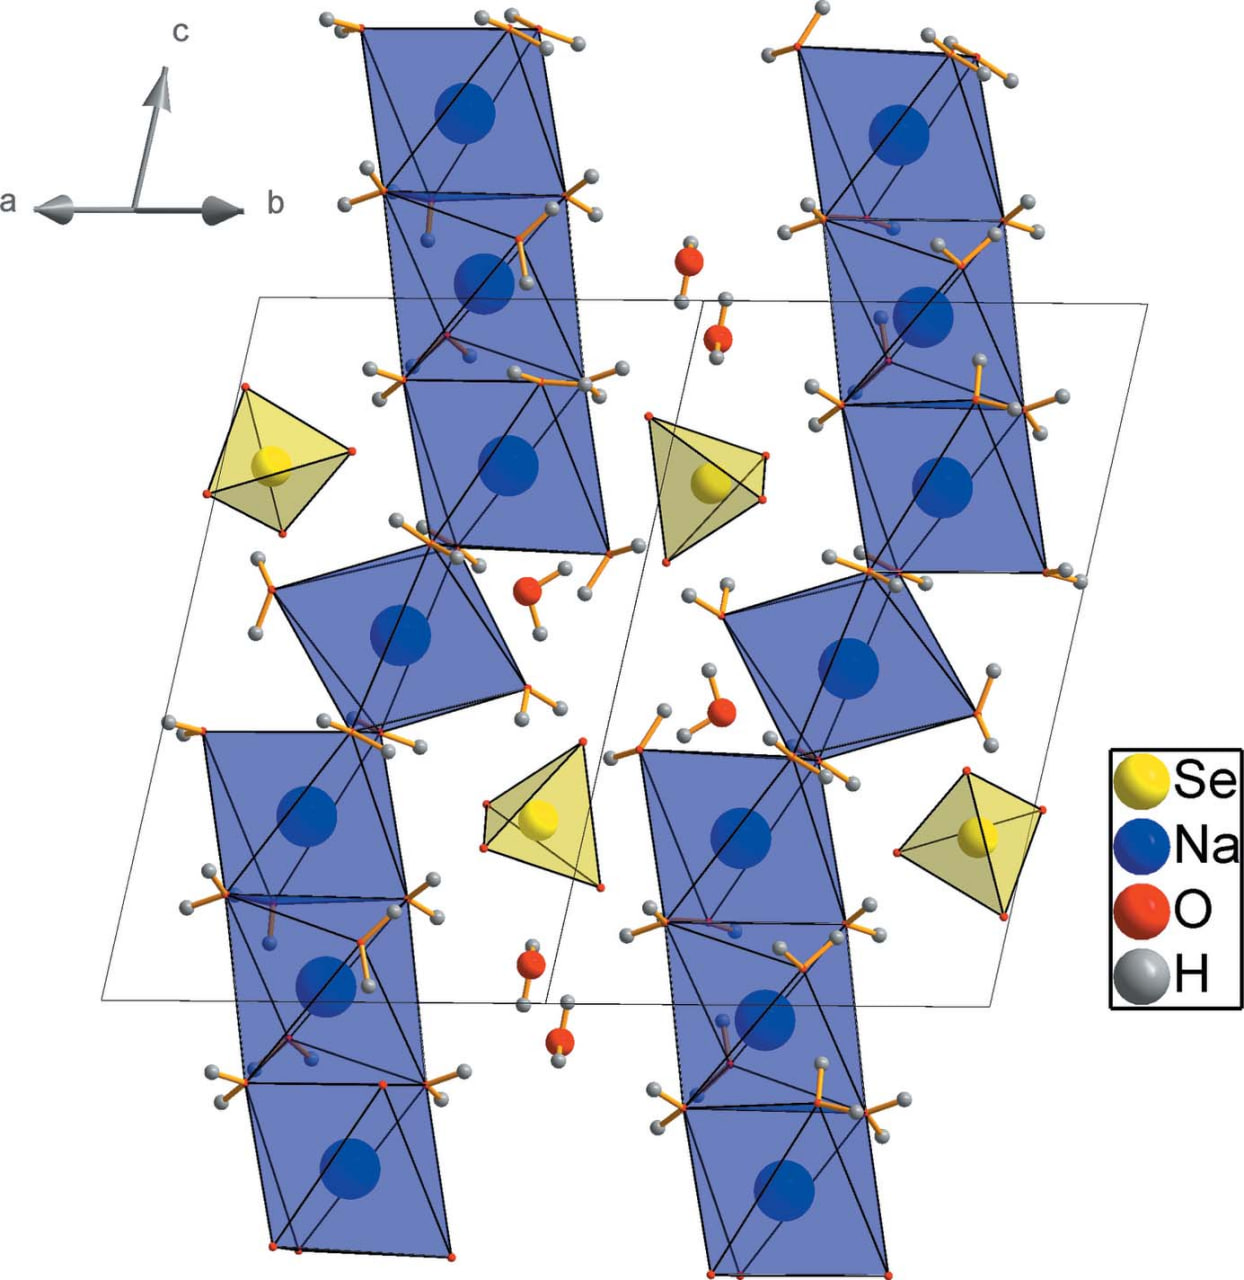
\includegraphics[width=0.4\linewidth]{img/Na2SeO4.10H2O-structure.jpg}
    \caption{Estrutura cristalina do \ce{Na2SeO4 . 10 H2O}, isomorfo ao \ce{Na2SO4 . 10 H2O}. São reportadas 4 unidades de fórmula em cada célula unitária. Fonte: \textcite{Kamburov2014}.}
    \label{fig:glauber-structure}
\end{figure}

É esse arranjo estrutural que permite ao \ce{Na2SO4} incorporar tantas moléculas de água em sua estrutura cristalina (tornando-se \ce{Na2SO4 . 10 H2O}) e, ainda assim, permanecer sólido à temperatura ambiente.
Essa característica enseja a pesquisa e aplicação desse sal em inúmeros processos, como, por exemplo, no controle térmico de painéis fotovoltaicos \cite{Gholami2023}, em sistemas de armazenamento a frio \cite{Xu2018} ou em processos de armazenamento termoquímico \cite{Donkers2015}. Também o efeito de se adicionar outros sais iônicos ao sal de Glauber para modificar suas propriedades tem sido estudado \cite{SankarDeepa2022}.

Para melhor analisar esse tipo de fenômeno, vem à luz as técnicas próprias da análise térmica, especialmente a Análise Termogravimétrica (TGA) e a Calorimetria Exploratória Diferencial (DSC), que submetem a amostra sólida a aquecimento controlado. Essas técnicas são amplamente empregadas na caracterização térmica de materiais: a TGA permite monitorar a variação de massa da amostra em função da temperatura; e a DSC, por sua vez, mostra o fluxo de calor associado aos eventos térmicos (desidratação, no caso em tela). A integração dos picos da DSC também fornece informações sobre a entalpia envolvida no processo --- $\Delta_{\text{desidr.}} H$ neste caso. \cite{Gabbott2008}

\textcite{Rens2012}, a partir das curvas TGA e DSC do sal de Glauber mostradas na \autoref{fig:glauber-tga-dsc}, demonstra que o \ce{Na2SO4 . 10H2O} se decompõe em \ce{Na2SO4} e água líquida a \qty{32}{\celsius}, mediante liberação das moléculas de \ce{H2O} do retículo cristalino, conforme corroborado por \textcite{Donkers2015}.

Analisando a TGA, \textcite{Rens2012} observa que a amostra apresenta uma perda de massa entre \qty{25}{\celsius} e \qty{60}{\celsius}, mas que tal perda de massa é acompanhada por um único pico endotérmico na DSC em $T = \qty{32}{\celsius}$.  O pico único observado na DSC indica que a desidratação propriamente dita ocorre em uma única etapa, \emph{id est}, toda a água quimicamente ligada é liberada em $T = \qty{32}{\celsius}$.

A constante perda de massa observada até os \qty{60}{\celsius} não indica, portanto, nova reação ou decomposição, mas pode ser explicada pela eliminação lenta da água condensada no interior da cápsula de medição, devido à restrição imposta pelo pequeno orifício da tampa, o que retarda sua saída. Esse fato é reforçado pela \autoref{fig:glauber-dsc-water}, que compara a DSC da amostra com a DSC da água pura na mesma configuração experimental. Dessa forma, a desidratação térmica do Sal de Glauber pode ser representada pela \autoref{eq:desidrata-glauber} ou, de forma mais precisa, pela \autoref{eq:desidrata-glauber2}. \cite{Rens2012}%
\begin{equation}%
    \ce{Na2SO4 . 10 H2O (s) <=>[\qty{32}{\celsius}] Na2SO4 (s) + 10 H2O (l)} \label{eq:desidrata-glauber}
\end{equation}%
\begin{equation}%
    \ce{Na2SO4 . 10 H2O (s) + $\Delta_{\text{desidr.}} H$ <=> Na2SO4 (s) + 10 H2O (l)} \label{eq:desidrata-glauber2}
\end{equation}%

\begin{figure}
    \centering
    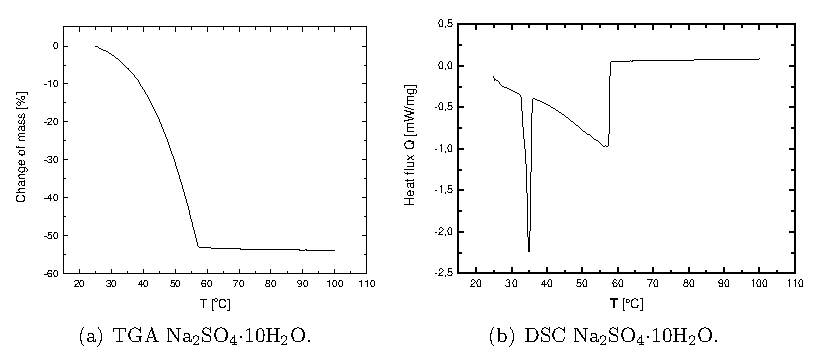
\includegraphics[width=\linewidth]{img/Glauber_TGA_DSC_Rens2012.pdf}
    \caption{Análise TGA e DSC do \ce{Na2SO4 . 10 H2O}, mostrando a desidratação térmica do sal a $T = \qty{32}{\celsius}$. Fonte: \textcite{Rens2012}.}
    \label{fig:glauber-tga-dsc}
\end{figure}

\begin{figure}
    \centering
    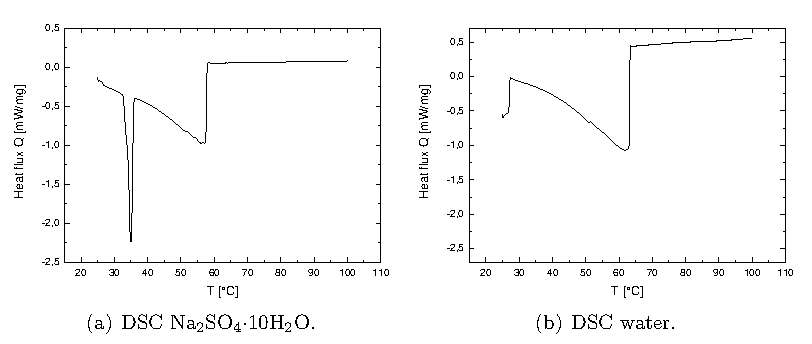
\includegraphics[width=\linewidth]{img/Glauber_Water_DSC_Rens2012.pdf}
    \caption{Análise DSC do \ce{Na2SO4 . 10 H2O} e da água, evidenciando que a perda de massa até $T \leq \qty{60}{\celsius}$ está relacionada à água, e não ao sal. Fonte: \textcite{Rens2012}.}
    \label{fig:glauber-dsc-water}
\end{figure}


\section{Físico-Química} \label{sec:fisquim}

\subsection{Descritores Moleculares}

Um dos métodos mais tradicionais em QSAR, a Análise Comparativa de Campo Molecular (CoMFA, do inglês \textit{Comparative Molecular Field Analysis}) \cite{Cramer1988}, consiste em otimizar a geometria da molécula de interesse e então colocá-la em uma caixa tridimensional, na qual uma sonda (como, por exemplo, um íon) percorrerá \( n \) pontos, sempre calculando as interações eletrostáticas e estéricas com a molécula. Esse procedimento é repetido para cada molécula do conjunto de \( m \) moléculas, gerando-se uma matriz \( A \in \mathbb{R}^{m \times n} \).

Define-se então um subespaço \( \mathcal{X} = C(A) = \text{span}\{A_1, A_2, \ldots, A_n\} \), em que \( C(A) \) é o espaço-coluna de \( A \) e \( A_i \) é a \( i \)-ésima coluna de \( A \). Posteriormente, partindo-se do entendimento que o subespaço \( \mathcal{X} \) também engloba ruídos e informações irrelevantes, gera-se uma nova base para um subespaço \( \mathcal{D} \subset \mathcal{X} \), com \( \dim(\mathcal{D}) < \dim(\mathcal{X}) \), aqui chamado de subespaço dos descritores selecionados, em alusão ao fato de que a hipótese central da QSAR é que esse subespaço é capaz de descrever satisfatoriamente o conjunto das moléculas.

\subsubsection{LQTA-QSAR}

Embora o formalismo proposto por \textcite{Hopfinger1997} tenha demonstrado bons resultados, sua metodologia de extração de descritores não contempla diretamente as interações eletrostáticas entre a molécula e o ambiente, limitando o realismo da modelagem. Visando superar essa limitação, \textcite{LQTAQSAR2009} propuseram, em 2009, o método LQTA-QSAR, que combina os princípios da CoMFA \cite{Cramer1988} com o formalismo 4D, incorporando descritores energéticos derivados do espaço conformacional da molécula.

No LQTA-QSAR, o Perfil de Amostragem Conformacional (CEP) da molécula é inserido em uma malha tridimensional. Cada ponto da malha é percorrido por uma sonda --- por exemplo, um íon \ce{NH3+} --- e, para cada posição, são calculadas as interações de Coulomb (\autoref{eq:coulomb}) e de Lennard-Jones (\autoref{eq:lj}) com todos os átomos do CEP. A \autoref{fig:LQTA-QSAR} ilustra esse processo para uma malha com resolução de 1 \AA.


\begin{figure}
    \centering
    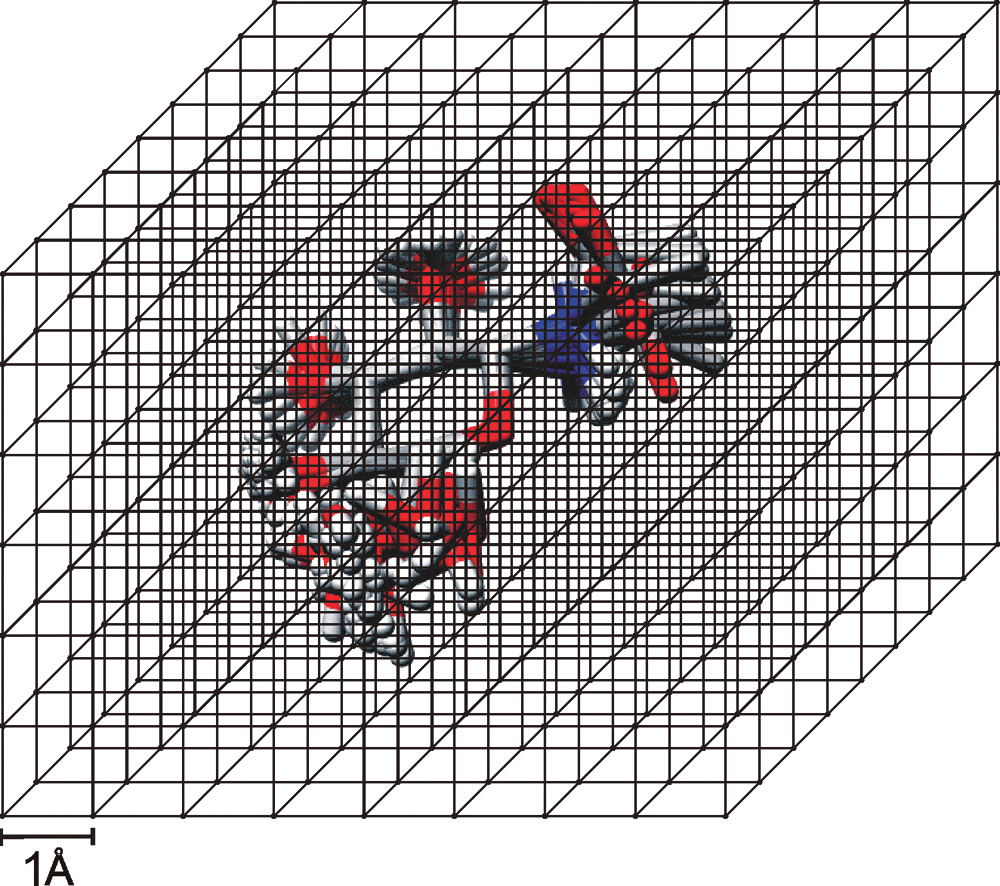
\includegraphics[width=0.5\textwidth]{img/LQTAQSAR_CEP.png}
    \caption{Exemplo de um perfil de amostragem conformacional (CEP) num grid do LQTA-QSAR de 1 \AA. Fonte: \textcite{LQTAQSAR2009}.}
    \label{fig:LQTA-QSAR}
  \end{figure}

Sejam $r_{ij}$ a distância entre o ponto $i$ da malha (onde está localizada a sonda) e o átomo $j$ do CEP; $\varepsilon$, a permissividade elétrica do meio; $n$, o número de conformações presentes no CEP; e $\{K_{ii}^{12}, K_{ii}^6, K_{jj}^{12}, K_{jj}^6\}$ os parâmetros do campo de força associados à sonda e aos átomos da molécula. As interações são dadas pelas expressões:

\begin{align}
    C &= \frac{1}{n} \sum_j \frac{q_i q_j}{4 \pi \varepsilon r_{ij}} \label{eq:coulomb} \\
    LJ &= \sum_j \left( \frac{K_{ij}^{12}}{r_{ij}^{12}} - \frac{K_{ij}^{6}}{r_{ij}^{6}} \right) \label{eq:lj} \\
    K_{ij}^{12} &= \sqrt{ \frac{K_{ii}^{12} \cdot K_{jj}^{12} }{n} } \\
    K_{ij}^{6} &= \sqrt{ \frac{K_{ii}^{6} \cdot K_{jj}^{6} }{n} }
\end{align}

Para cada CEP, gera-se um vetor de descritores $\vec{x}_i \in \RR^{2m}$, representando as energias calculadas nos pontos da malha. Considerando uma caixa cúbica de aresta $a$ e resolução de 1 \AA, são amostrados $a^3$ pontos, cada um com duas energias (Coulomb e Lennard-Jones), resultando em uma matriz de descritores $X \in \RR^{2a^3 \times m}$.

Apesar de eficiente, essa abordagem apresenta uma limitação importante: a malha pode conter pontos muito próximos aos átomos do CEP, fazendo $r_{ij} \to 0$. Nessas situações, \eqref{eq:coulomb} e \eqref{eq:lj} tendem ao infinito ($\lim_{r_{ij} \to 0} C = \lim_{r_{ij} \to 0} LJ = \infty$), produzindo valores de energia não realistas que comprometem a qualidade dos descritores e, consequentemente, a performance do modelo.

Em resumo, o LQTA-QSAR permite a amostragem do espaço conformacional de uma molécula por meio de uma malha tridimensional, associando a cada ponto vetores de energia obtidos a partir de interações físico-químicas simuladas com uma sonda. Esses vetores energéticos são então utilizados como descritores para a modelagem QSAR. Contudo, a presença de pontos com interações singularmente elevadas pode introduzir variáveis irrelevantes e comprometer a robustez estatística do modelo.

\subsubsection{LQTAGridHull — Amostragem Filtrada por Geometria Convexa}

Uma das principais limitações do LQTA-QSAR e de métodos relacionados, como o CoMFA, reside no fato de que a sonda pode ser posicionada muito próxima --- ou mesmo no interior --- de um átomo do CEP. Nessas condições, as interações de Coulomb e Lennard-Jones calculadas nos pontos da malha tendem ao infinito ($r_{ij} \to 0$), o que gera descritores fisicamente inverossímeis, reduz a robustez estatística dos modelos e compromete sua interpretabilidade.

Para mitigar esse problema, \textcite{Tenorio2018} propuseram o método \textit{LQTAGridHull}, que introduz o conceito de fecho convexo na etapa de amostragem dos descritores. Em geometria computacional, o \emph{fecho convexo} $\mathcal{F}(X)$ de um conjunto de pontos $X \subset \RR^d$ é definido como o menor conjunto convexo que o contém. Formalmente:

\begin{equation} \label{eq:def-convex-hull}
\mathcal{F}(X) = \left\{ \sum_{i=1}^{k} \lambda_i x_i \ \middle| \ x_i \in X, \lambda_i \ge 0, \sum_{i=1}^{k} \lambda_i = 1 \right\}
\end{equation}

A \autoref{fig:convex_hull_2d} ilustra esse conceito em duas dimensões, com os pontos de um conjunto $X \subset \RR^2$ (em azul) e seu fecho convexo $\mathcal{F}(X)$ (delineado pela linha vermelha).

\begin{figure}
  \centering
  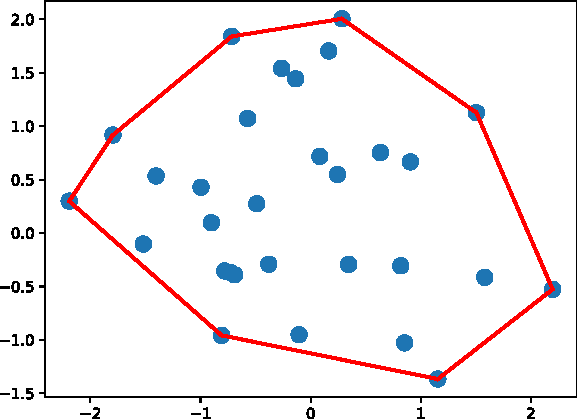
\includegraphics[width=0.5\textwidth]{img/convex_hull_2d.pdf}
  \caption{Exemplo de fecho convexo $\mathcal{F}(X)$ (linha vermelha) do conjunto $X \subset \RR^2$ (pontos azuis). Fonte: \textcite{Tenorio2018}.}
  \label{fig:convex_hull_2d}
\end{figure}

No contexto da 4D-QSAR, cada átomo de cada conformação no CEP é representado como um ponto $x_i \in X$, em que $X \subset \RR^3$. O fecho convexo tridimensional desses pontos, denotado por $\mathcal{H}(X)$, corresponde à menor região convexa que os contém, servindo como uma barreira natural para restringir a amostragem de descritores às regiões externas da densidade atômica.

A superfície $\partial \mathcal{H}(X)$ é então expandida radialmente por uma distância $r_0$, originando uma nova superfície $\mathcal{H}'(X)$:

\begin{equation}
\mathcal{H}'(X) = \left\{ x + r_0 \cdot \hat{n}_x \mid x \in \partial \mathcal{H}(X), \hat{n}_x \text{ é a normal externa em } x \right\}
\end{equation}

A partir dessa superfície inicial, define-se uma sequência de cascas esféricas com incrementos radiais $\Delta_r$:

\begin{equation}
\mathcal{H}^{(k)}(X) = \left\{ x + (r_0 + k \Delta_r) \cdot \hat{n}_x \right\}, \quad k = 0, \dots, l-1
\end{equation}

O número total de cascas, $l$, é dado por \eqref{eq:max-num-of-r-steps}. Em cada casca, define-se uma malha esférica com espaçamento angular $\Delta_\alpha$ em coordenadas esféricas $(\theta, \phi)$, resultando no número total de pontos amostrados, calculado em \eqref{eq:max-num-of-points}.

\begin{equation}
l = 1 + \left\lfloor \frac{r_{\mathrm{max}} - r_0}{\Delta_r} \right\rfloor
\label{eq:max-num-of-r-steps}
\end{equation}

\begin{equation}
Z = l \left[ \left\lfloor \frac{360}{\Delta_\alpha} \right\rfloor \cdot \left\lfloor \frac{180}{\Delta_\alpha} \right\rfloor - 2 \left( \left\lfloor \frac{180}{\Delta_\alpha} \right\rfloor - 1 \right) \right]
\label{eq:max-num-of-points}
\end{equation}

Para cada ponto $z_j$ da malha, as interações com os átomos do CEP são calculadas por:

\begin{align*}
d_j^{\text{C}} &= \sum_{i=1}^{N} \frac{q_i q_j}{4 \pi \varepsilon_0 \, \|z_j - x_i\|} \\
d_j^{\text{LJ}} &= \sum_{i=1}^{N} \left( \frac{A_{ij}}{\|z_j - x_i\|^{12}} - \frac{B_{ij}}{\|z_j - x_i\|^6} \right)
\end{align*}



\section{Inteligência Artificial} \label{sec:ia}

A Inteligência Artificial é um campo da ciência da computação que se dedica a desenvolver sistemas capazes de executar tarefas que normalmente exigiriam inteligência humana. Desde a sua origem, a IA tem se caracterizado por uma série de marcos teóricos e práticos que, juntos, vêm moldando a forma como o ser humano interage com a tecnologia e com o mundo moderno.

Embora a popularização do termo seja recente e esteja frequentemente associada ao surgimento da \emph{Inteligência Artificial Generativa}, marcado pelo lançamento de modelos de linguagem como o \emph{ChatGPT}, os primeiros estudos nesta área na verdade remontam à segunda metade do século XX.

Em 1950, Alan Turing publica o seu artigo intitulado \citetitle{turing1950}, no qual se concentra na definição e no estudo da ``inteligência''. Nesse trabalho, o amplamente considerado ``pai da computação'' propõe uma questão que, até o momento, não escaparia da esfera filosófica: \textbf{``As máquinas podem pensar?''} \cite{turing1950}.

Para responder a essa difícil e até então inexplorada pergunta, \citeauthor{turing1950} propõe um experimento que ficaria conhecido como o ``Teste de Turing''. A ideia é simples: um juiz humano interage com duas entidades, uma máquina e um ser humano, sem saber qual é qual. Se o juiz não for capaz de distinguir entre as respostas da máquina e do humano, então a máquina pode ser considerada ``inteligente''.

Esse trabalho não apenas inaugurou uma nova forma de pensar sobre a interação homem--máquina, mas também lançou as bases para a formalização do estudo dessa nova área.

Pouco mais tarde, ainda na década de 1950, o termo ``inteligência artificial'' é então cunhado pelo Prof. John McCarthy, hoje Professor Emérito de Ciência da Computação da Universidade Stanford, quem responde ao questionamento \emph{``o que é inteligência artificial?''} com as seguintes palavras:

\begin{citacao}[english]
   É a ciência e a engenharia de criar máquinas inteligentes, especialmente programas de computador inteligentes. Está relacionada à tarefa semelhante de usar computadores para entender a inteligência humana, mas a IA não precisa se limitar a métodos que sejam biologicamente observáveis \cite[tradução própria]{mccarthy2007}.
\end{citacao}

Poucos anos depois, em 1956, a Conferência de Dartmouth reuniu um grupo de pioneiros --- entre eles Marvin Minsky, Claude Shannon e Herbert Simon --- e estabeleceu o ponto de partida formal para a pesquisa em IA. Esse encontro não só popularizou o termo, mas também incentivou o desenvolvimento de métodos simbólicos e heurísticos para resolver problemas complexos.

